% ============================================================
%  CHAPTER 2: Goal Setting and Goal-Based Investing
%  Part of: Beginner's Guide to Selecting Mutual Funds
%  Sources: Your Everyday Guide, CA Rachana Ranade (SMART Goals),
%           IMD Learn, Finology (Pranjal Kamra), Udayan Adhye
% ============================================================

\documentclass[12pt,a4paper]{article}

% ── Packages ─────────────────────────────────────────────────
\usepackage[utf8]{inputenc}
\usepackage[T1]{fontenc}
\usepackage[a4paper, top=25mm, bottom=25mm,
            left=22mm, right=22mm]{geometry}
\usepackage{amsmath,amssymb}
\usepackage{xcolor}
\usepackage{tcolorbox}
\tcbuselibrary{skins,breakable,theorems}
\usepackage{enumitem}
\usepackage{booktabs}
\usepackage{tabularx}
\usepackage{array}
\newcolumntype{L}[1]{>{\raggedright\arraybackslash}p{#1}}
\newcolumntype{B}[1]{>{\bfseries\raggedright\arraybackslash}p{#1}}
\usepackage{multicol}
\usepackage{pifont}
\usepackage{tikz}
\usetikzlibrary{arrows.meta,shapes,positioning,fit,
                backgrounds,calc,decorations.text}
\usepackage{hyperref}
\hypersetup{colorlinks=true,linkcolor=NavyBlue,urlcolor=NavyBlue}
\usepackage{parskip}
\usepackage{mdframed}
\usepackage{colortbl}
\usepackage{needspace}

% ── Rupee symbol ─────────────────────────────────────────────
\newcommand{\rupee}{\ifmmode\text{Rs.}\else Rs.\@\fi}

% ── Colour palette ───────────────────────────────────────────
\definecolor{PrimaryBlue}{HTML}{1A3C6E}
\definecolor{AccentTeal}{HTML}{00897B}
\definecolor{AccentOrange}{HTML}{E65100}
\definecolor{AccentPurple}{HTML}{6A1B9A}
\definecolor{AccentGold}{HTML}{F9A825}
\definecolor{AccentRed}{HTML}{B71C1C}
\definecolor{AccentGreen}{HTML}{2E7D32}
\definecolor{LightBlue}{HTML}{E3F2FD}
\definecolor{LightGreen}{HTML}{E8F5E9}
\definecolor{LightOrange}{HTML}{FFF3E0}
\definecolor{LightRed}{HTML}{FFEBEE}
\definecolor{LightPurple}{HTML}{F3E5F5}
\definecolor{LightGold}{HTML}{FFFDE7}
\definecolor{SoftGray}{HTML}{F5F5F5}
\definecolor{DarkGray}{HTML}{37474F}
\definecolor{MidGray}{HTML}{78909C}
\definecolor{ShortTerm}{HTML}{1565C0}
\definecolor{MedTerm}{HTML}{558B2F}
\definecolor{LongTerm}{HTML}{6A1B9A}
\definecolor{VeryLong}{HTML}{B71C1C}
\definecolor{SMARTblue}{HTML}{0277BD}

% ── tcolorbox environments ────────────────────────────────────
\tcbset{
  base/.style={
    arc=4pt, boxrule=0.8pt, left=8pt, right=8pt,
    top=6pt, bottom=6pt, breakable
  }
}

\newtcolorbox{conceptbox}[2][]{
  base, colback=LightBlue, colframe=PrimaryBlue,
  fonttitle=\bfseries\color{white}, title={#2}, #1,
  attach boxed title to top left={yshift=-2mm,xshift=4mm},
  boxed title style={colback=PrimaryBlue,arc=3pt,boxrule=0pt}
}

\newtcolorbox{definitionbox}[2][]{
  base, colback=LightGreen, colframe=AccentTeal,
  fonttitle=\bfseries\color{white},
  title={\ding{228}\;#2}, #1,
  attach boxed title to top left={yshift=-2mm,xshift=4mm},
  boxed title style={colback=AccentTeal,arc=3pt,boxrule=0pt}
}

\newtcolorbox{examplebox}[2][]{
  base, colback=LightOrange, colframe=AccentOrange,
  fonttitle=\bfseries\color{white},
  title={\ding{42}\;#2}, #1,
  attach boxed title to top left={yshift=-2mm,xshift=4mm},
  boxed title style={colback=AccentOrange,arc=3pt,boxrule=0pt}
}

\newtcolorbox{warningbox}[1][]{
  base, colback=LightRed, colframe=AccentRed,
  fonttitle=\bfseries\color{white},
  title={\ding{54}\;Important Caution}, #1,
  attach boxed title to top left={yshift=-2mm,xshift=4mm},
  boxed title style={colback=AccentRed,arc=3pt,boxrule=0pt}
}

\newtcolorbox{keybox}[1][]{
  base, colback=LightPurple, colframe=AccentPurple,
  fonttitle=\bfseries\color{white},
  title={\ding{166}\;Key Takeaway}, #1,
  attach boxed title to top left={yshift=-2mm,xshift=4mm},
  boxed title style={colback=AccentPurple,arc=3pt,boxrule=0pt}
}

\newtcolorbox{cheatsheet}[1][]{
  base, colback=SoftGray, colframe=DarkGray,
  fonttitle=\bfseries\color{white},
  title={\ding{113}\;Quick Reference Cheat Sheet}, #1,
  attach boxed title to top left={yshift=-2mm,xshift=4mm},
  boxed title style={colback=DarkGray,arc=3pt,boxrule=0pt}
}

\newtcolorbox{stepbox}[2][]{
  base, colback=#1!8, colframe=#1,
  fonttitle=\bfseries\color{white},
  title={#2},
  attach boxed title to top left={yshift=-2mm,xshift=4mm},
  boxed title style={colback=#1,arc=3pt,boxrule=0pt}
}

% ── Section styling ───────────────────────────────────────────
\usepackage{titlesec}
\titleformat{\section}[block]
  {\Large\bfseries\color{PrimaryBlue}}
  {\thesection.}{0.6em}{}[{\color{PrimaryBlue}\titlerule[1.5pt]}]

\titleformat{\subsection}[block]
  {\large\bfseries\color{AccentTeal}}
  {\thesubsection.}{0.5em}{}

\titleformat{\subsubsection}[runin]
  {\normalsize\bfseries\color{DarkGray}}
  {\thesubsubsection.}{0.4em}{}[.\quad]

\setlist[itemize]{leftmargin=*,topsep=3pt,itemsep=2pt}
\setlist[enumerate]{leftmargin=*,topsep=3pt,itemsep=2pt}

% ── Smart letter box ─────────────────────────────────────────
\newcommand{\smartletter}[3]{%
  \begin{tcolorbox}[base,colback=#1!8,colframe=#1,
    title={\Large\bfseries\color{white}#2\ \normalsize\bfseries\color{white}---\ #3},
    fonttitle=\bfseries,
    attach boxed title to top left={yshift=-2mm,xshift=4mm},
    boxed title style={colback=#1,arc=3pt,boxrule=0pt}]}

\newcommand{\smartheading}[4]{%
  \begingroup
  \setlength{\fboxsep}{4pt}%
  \noindent\colorbox{#1}{%
    \parbox{\dimexpr\linewidth-2\fboxsep\relax}{%
      \Large\bfseries\color{#4}#2\ \normalsize\bfseries---\ #3\strut%
    }%
  }%
  \par\endgroup\medskip
}

% ── Document ─────────────────────────────────────────────────
\begin{document}

% ── Title block ──────────────────────────────────────────────
\begin{tcolorbox}[
  enhanced, arc=6pt, boxrule=0pt,
  colback=PrimaryBlue, colframe=PrimaryBlue,
  left=14pt, right=14pt, top=14pt, bottom=14pt
]
  {\color{white}\Huge\bfseries Chapter 2}\\[4pt]
  {\color{white!80!PrimaryBlue}\Large\itshape
   Beginner's Guide to Selecting Mutual Funds}\\[10pt]
  {\color{white}\rule{\linewidth}{0.6pt}}\\[8pt]
  {\color{white}\LARGE\bfseries
   Goal Setting \& Goal-Based Investing}\\[6pt]
  {\color{white!75!PrimaryBlue}\normalsize
   Turning financial dreams into funded, time-bound plans ---
   and choosing the right mutual fund for each one.}
\end{tcolorbox}

\vspace{4mm}

% ── Opening motivation ────────────────────────────────────────
\begin{conceptbox}{Why This Chapter Is the Heart of Financial Planning}
Most investors think investing is simply about putting money somewhere and waiting to ``become rich.'' But here is a better question: \textit{Become rich for what?} What will you do with that money? When will you need it? How much will you need?

Without answers to these questions, you are driving without a destination --- you may cover a lot of ground but arrive nowhere useful. This chapter gives you the complete framework: how to \textbf{set goals}, how to \textbf{prioritize them}, how to \textbf{account for inflation}, how to \textbf{match each goal to the right mutual fund category}, and how to \textbf{calculate your exact SIP amount}.
\end{conceptbox}

\vspace{2mm}

% ─────────────────────────────────────────────────────────────
\section{Growth-Based vs.\ Goal-Based Investing: The Core Distinction}
% ─────────────────────────────────────────────────────────────

Before learning \textit{how} to set goals, you must understand \textit{why} goal-based investing is fundamentally different from the way most people invest.

\subsection{Growth-Based Investing}

\begin{definitionbox}{Growth-Based Investing}
\textbf{Growth-based investing} focuses on one objective: \textbf{maximising the growth of your capital} by beating the market. The measure of success is how much \textit{Alpha} your portfolio generates --- that is, how much your returns \textit{exceed} the market's average return.
\end{definitionbox}

\begin{itemize}
  \item \textbf{The goal:} Beat the benchmark (e.g.\ Nifty 50) by as large a margin as possible.
  \item \textbf{The metric of success:} Alpha generated $=$ Portfolio return $-$ Market return.
  \item \textbf{The philosophy:} ``More return is always better, regardless of my life situation.''
  \item \textbf{Typical allocation:} Heavier in equity (e.g.\ 60\% equity, 40\% debt/other).
  \item \textbf{Best suited for:} Investors in their late 20s or early 30s with few responsibilities, a long time horizon, and no critical short-term financial obligations.
\end{itemize}

\subsection{Goal-Based Investing}

\begin{definitionbox}{Goal-Based Investing}
\textbf{Goal-based investing} organises every rupee you invest around a specific personal life goal --- a child's education, buying a home, retirement, a vacation. The measure of success is \textbf{whether you have the right amount of money at exactly the right time}, not whether you beat the market.
\end{definitionbox}

\begin{itemize}
  \item \textbf{The goal:} Fund each specific life milestone on schedule.
  \item \textbf{The metric of success:} Did I accumulate the required corpus by the required date?
  \item \textbf{The philosophy:} ``The \textit{minimum} investment needed to meet my goal is the correct investment --- not the maximum possible risk.''
  \item \textbf{Typical allocation:} More conservative, and \textit{varies by goal}. Conservative for near-term goals, aggressive only for distant ones.
  \item \textbf{Best suited for:} Anyone who has crossed 34--35 years of age, has specific financial responsibilities (home loan, children, retirement), or simply wants a clear, structured financial life at any age.
\end{itemize}

\subsection{The Critical Difference: Akshay's Story}

\begin{examplebox}{The Same Portfolio, Two Completely Different Outcomes}
Let us say \textbf{Akshay} needs \rupee{}11 lakh \textit{next year} for his child's college admission. He has \rupee{}10 lakh invested in equities, and he expects at least 10\% growth.

\medskip
Instead, the market falls 20\%. Because Akshay has a diversified portfolio, his loss is only 10\%. His portfolio is now worth \rupee{}9 lakh.

\medskip
\textbf{From a growth-based perspective:} Akshay ``won'' --- his portfolio only fell 10\% while the market fell 20\%. He generated +10\% Alpha. Success!

\medskip
\textbf{From a goal-based perspective:}
\begin{itemize}
  \item He \textit{expected} \rupee{}11 lakh. He \textit{received} \rupee{}9 lakh.
  \item His real loss is not 10\% --- it is 22\%.
  \item (\rupee{}11 lakh was the target; \rupee{}9 lakh is what he got; gap = \rupee{}2 lakh $\div$ \rupee{}9 lakh $\approx$ 22\%)
  \item His child may not be able to enrol in the planned college. The goal \textbf{failed}.
\end{itemize}

\medskip
\textbf{Lesson:} Akshay chose the wrong \textit{type} of investment for a short-term, non-negotiable goal. A goal-based investor would have placed this money in a safe debt instrument 1--2 years before the deadline --- regardless of market conditions.
\end{examplebox}

\begin{keybox}
Growth-based investing asks: \textit{``Am I beating the market?''}\\
Goal-based investing asks: \textit{``Will I have the right amount of money when I need it?''}\\[4pt]
These are two completely different questions, and they lead to very different investment decisions.
\end{keybox}

% ─────────────────────────────────────────────────────────────
\section{Step 1 --- Financial Goal Setting: The Foundation}
% ─────────────────────────────────────────────────────────────

\begin{conceptbox}{What Is Financial Goal Setting?}
\textbf{Financial goal setting} is the process of identifying what you want to achieve with your money, attaching a specific rupee amount and a specific deadline to each objective, and then planning your savings and investments \textit{systematically} to reach each one on time. It is the GPS system of your financial life.
\end{conceptbox}

Without defined goals, investing is just noise. With goals, every SIP you run has a name and a purpose. You know exactly why you are investing, for how long, and how much.

\subsection{Types of Financial Goals}

Goals are generally divided into three horizons based on \textbf{how far away they are}. This classification directly determines which investment instrument is appropriate.

\vspace{3mm}

\begin{center}
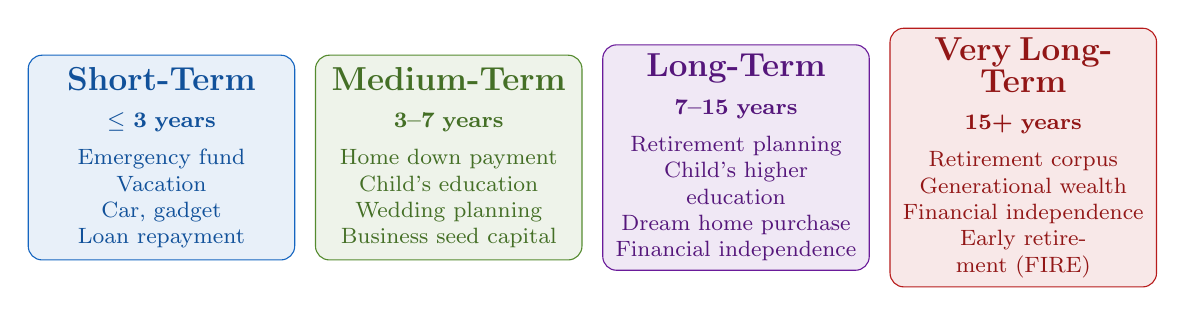
\begin{tikzpicture}[
  tbox/.style={rectangle, rounded corners=5pt, draw=#1, fill=#1!10,
               text=#1!80!black, text width=3.15cm, minimum width=3.15cm,
               minimum height=2.6cm, align=center, font=\footnotesize}
]
  \node[tbox=ShortTerm] (st) {
    \textbf{\large Short-Term}\\[4pt]
    \textbf{$\leq$ 3 years}\\[4pt]
    Emergency fund\\
    Vacation\\
    Car, gadget\\
    Loan repayment
  };
  \node[tbox=MedTerm, right=0.25cm of st] (mt) {
    \textbf{\large Medium-Term}\\[4pt]
    \textbf{3--7 years}\\[4pt]
    Home down payment\\
    Child's education\\
    Wedding planning\\
    Business seed capital
  };
  \node[tbox=LongTerm, right=0.25cm of mt] (lt) {
    \textbf{\large Long-Term}\\[4pt]
    \textbf{7--15 years}\\[4pt]
    Retirement planning\\
    Child's higher education\\
    Dream home purchase\\
    Financial independence
  };
  \node[tbox=VeryLong, right=0.25cm of lt] (vl) {
    \textbf{\large Very Long-Term}\\[4pt]
    \textbf{15+ years}\\[4pt]
    Retirement corpus\\
    Generational wealth\\
    Financial independence\\
    Early retirement (FIRE)
  };
\end{tikzpicture}
\end{center}

\vspace{4mm}

% ─────────────────────────────────────────────────────────────
\section{Step 2 --- The SMART Goal Framework}
% ─────────────────────────────────────────────────────────────

A vague wish is not a goal. ``I want to be rich'' is not a plan. The \textbf{SMART framework} transforms any financial dream into a precise, actionable investment objective. Each letter represents a mandatory quality that every goal must have.

\vspace{3mm}

% S
\Needspace{9\baselineskip}
\begin{tcolorbox}[base, colback=SMARTblue!8, colframe=SMARTblue]
\smartheading{SMARTblue}{S}{Specific: Know Exactly What You Want}{white}

A goal must be \textbf{clearly defined}. Vague aspirations give you no direction. You must state precisely what you want to achieve and identify the concrete steps required.

\medskip
\textbf{Questions to ask yourself:}
\begin{itemize}
  \item What exactly do I want to achieve?
  \item What specific steps will get me there?
\end{itemize}

\medskip
\begin{tabular}{p{0.44\linewidth} p{0.44\linewidth}}
\textbf{\color{AccentRed}Not Specific (Vague)} & \textbf{\color{AccentGreen}Specific (Clear)}\\
``I want to be financially free'' & ``I want to retire at age 50 with a monthly income of \rupee{}1 lakh''\\[4pt]
``I want to buy a car'' & ``I want to buy a Maruti Brezza (approx.\ \rupee{}12 lakh today) in 4 years''\\[4pt]
``I want to save money'' & ``I want to build an emergency fund of 6 months of expenses (\rupee{}3 lakh) within 18 months''\\
\end{tabular}
\end{tcolorbox}

\vspace{3mm}

% M
\Needspace{9\baselineskip}
\begin{tcolorbox}[base, colback=AccentTeal!8, colframe=AccentTeal]
\smartheading{AccentTeal}{M}{Measurable: Attach a Number to It}{white}

If you cannot \textbf{measure} your goal, you cannot track progress or know when you have succeeded. Every financial goal needs a specific rupee figure.

\medskip
\textbf{Questions to ask yourself:}
\begin{itemize}
  \item How much money do I need exactly?
  \item How will I track whether I am on course?
\end{itemize}

\medskip
\textbf{In practice:} ``I want my child to go to a good college'' becomes ``I need \rupee{}25 lakh (in today's value) for my child's undergraduate education in 12 years.'' This gives you something to calculate a SIP around.

\medskip
\textbf{The measurable number also tells you your monthly SIP.} Once you know the target amount and the timeline, an online SIP calculator immediately tells you how much to invest each month.
\end{tcolorbox}

\vspace{3mm}

% A
\Needspace{9\baselineskip}
\begin{tcolorbox}[base, colback=AccentGold!15, colframe=AccentGold]
\smartheading{AccentGold}{A}{Achievable: Be Honest About What Is Feasible}{DarkGray}

Your goals must be \textbf{realistic} given your current income, expenses, and skills. Overambitious goals set without grounding lead to discouragement and abandonment.

\medskip
\textbf{Three key questions to determine achievability:}
\begin{enumerate}
  \item Do I have the necessary financial resources (income / savings) right now?
  \item If not, can I acquire them --- through a salary increase, reducing expenses, or a second income?
  \item Am I trying to do too many things at once? (Buying a house \textit{and} a car \textit{and} taking a vacation in the same year is rarely achievable simultaneously.)
\end{enumerate}

\medskip
\textbf{The adjustment rule:} If a goal is currently not achievable, do not abandon it --- adjust either the \textit{target amount} (choose a less expensive option), the \textit{timeline} (give yourself more years), or both. A goal planner or app can help you model these adjustments.
\end{tcolorbox}

\vspace{3mm}

% R
\Needspace{9\baselineskip}
\begin{tcolorbox}[base, colback=AccentOrange!8, colframe=AccentOrange]
\smartheading{AccentOrange}{R}{Relevant: Make Sure It Truly Matters to You}{white}

A goal that is not \textbf{aligned with your values} will not motivate you to stay disciplined over years. The ``Why'' behind a goal is what keeps you invested during market downturns instead of panic-selling.

\medskip
\textbf{Questions to ask yourself:}
\begin{itemize}
  \item Why do I want to achieve this goal?
  \item Does this goal matter enough to me personally that I will sustain a monthly SIP for 10 years?
  \item Am I pursuing this goal because \textit{I} want it, or because of social pressure?
\end{itemize}

\medskip
\textbf{Example of relevance test:} If you are investing for a luxury car but do not actually care about cars, you will likely stop your SIP when the market dips. However, if the goal is your child's education --- something you would sacrifice almost anything for --- you will hold through every market cycle.
\end{tcolorbox}

\vspace{3mm}

% T
\Needspace{9\baselineskip}
\begin{tcolorbox}[base, colback=AccentPurple!8, colframe=AccentPurple]
\smartheading{AccentPurple}{T}{Time-Bound: Every Goal Needs a Deadline}{white}

Without a \textbf{deadline}, a goal is just a dream. Time-binding your goal serves two critical functions in investing: (1) it determines \textit{how urgent} your planning needs to be, and (2) it determines \textit{which type of instrument} is appropriate.

\medskip
\textbf{Question to ask yourself:}
\begin{itemize}
  \item When exactly do I need this money? (Month and year, not just ``in a few years'')
\end{itemize}

\medskip
\textbf{Examples:}
\begin{itemize}
  \item ``I want to be financially independent by age 45'' --- this gives you a specific number of years, from which you calculate how aggressively you must invest.
  \item ``I need \rupee{}50 lakh for a home down payment by March 2029'' --- exact date, exact amount. You can now calculate your SIP immediately.
\end{itemize}

\medskip
\textbf{The timeline also determines your fund category} (as explained in Section 5). A 2-year deadline means a liquid/debt fund. A 15-year deadline means an aggressive equity fund.
\end{tcolorbox}

\vspace{3mm}

\begin{keybox}
A well-formed SMART financial goal looks like this:

\medskip
\textit{``I want to accumulate \rupee{}40 lakh (inflation-adjusted) for my daughter's undergraduate education, which begins in 14 years (July 2039). I will achieve this by investing \rupee{}X/month in a flexi-cap mutual fund via SIP, reviewed annually.''}

\medskip
Notice it has: a specific amount, a measurable SIP target, a realistic plan, a clear motivation (daughter's education), and an exact deadline.
\end{keybox}

% ─────────────────────────────────────────────────────────────
\section{Step 3 --- Accounting for Inflation: The Most Ignored Step}
% ─────────────────────────────────────────────────────────────

\begin{warningbox}
\textbf{The most common mistake in goal planning:} Calculating target amounts in \textit{today's prices} without adjusting for inflation. If your child's engineering degree costs \rupee{}15 lakh today and you are planning for 12 years from now, you do \textbf{not} need \rupee{}15 lakh. You need significantly more.
\end{warningbox}

\subsection{Why Inflation Matters in Goal Calculation}

India's average long-term inflation rate is approximately \textbf{6--7\% per year}. This means that whatever something costs today, it will cost roughly double in 10--12 years (this is the ``Rule of 72'' applied to inflation: $72 \div 6 = 12$ years to double).

\subsection{The Rule of 72 for Inflation}

\begin{definitionbox}{Rule of 72}
Divide 72 by the assumed annual inflation rate. The result is the approximate number of years it takes for prices to \textbf{double}.

$$\text{Years to double} \approx \frac{72}{\text{Inflation Rate (\%)}}$$

At 6\% inflation: $72 \div 6 = 12$ years for prices to double.
At 7\% inflation: $72 \div 7 \approx 10$ years for prices to double.
\end{definitionbox}

\subsection{How to Calculate Your Inflation-Adjusted Target}

\textbf{Method:} Take the current cost of your goal and increase it by 6--7\% compounded each year until your target date.

\begin{examplebox}{Car Purchase in 5 Years}
\textbf{Goal:} Buy a car currently priced at \rupee{}10 lakh. Timeline: 5 years. Assumed inflation: 7\%.

\medskip
\textbf{Calculation} (compounding 7\% annually):
\begin{align*}
\text{Year 1:} &\quad 10{,}00{,}000 \times 1.07 = 10{,}70{,}000\\
\text{Year 2:} &\quad 10{,}70{,}000 \times 1.07 \approx 11{,}45{,}000\\
\text{Year 3:} &\quad 11{,}45{,}000 \times 1.07 \approx 12{,}25{,}000\\
\text{Year 4:} &\quad 12{,}25{,}000 \times 1.07 \approx 13{,}10{,}000\\
\text{Year 5:} &\quad 13{,}10{,}000 \times 1.07 \approx 14{,}00{,}000
\end{align*}

You do \textbf{not} need \rupee{}10 lakh. You need approximately \textbf{\rupee{}14 lakh} in 5 years. This \rupee{}14 lakh --- not \rupee{}10 lakh --- is the number you put into your SIP calculator.
\end{examplebox}

\begin{examplebox}{Child's Education in 12 Years}
\textbf{Goal:} Engineering degree currently costing \rupee{}15 lakh. Timeline: 12 years. Inflation: 6\%.

\medskip
Using Rule of 72: at 6\%, prices double in 12 years.

Therefore, the future cost $\approx 2 \times \rupee{}15$ lakh $=$ \textbf{\rupee{}30 lakh}.

(More precisely: $15 \times (1.06)^{12} \approx \rupee{}30.2$ lakh.)

\medskip
If you had planned for only \rupee{}15 lakh, you would be about \rupee{}15 lakh short --- essentially funding only half the degree.
\end{examplebox}

\vspace{2mm}

\textbf{Practical tools:} Many free online goal calculators are available where you simply enter the current cost of your goal, the number of years, and the inflation rate (6--7\%), and they tell you the exact inflation-adjusted target amount.

% ─────────────────────────────────────────────────────────────
\section{Step 4 --- Calculating Net Worth: Knowing Where You Stand}
% ─────────────────────────────────────────────────────────────

Before you can plan how much to invest, you need to know your current financial position. This is captured by your \textbf{net worth}.

\begin{definitionbox}{Net Worth}
$$\text{Net Worth} = \text{Total Assets} - \text{Total Liabilities}$$

\textbf{Assets} are things that add financial value: investments, property, savings account balance, gold, EPF balance.\\
\textbf{Liabilities} are things that reduce financial value: home loan outstanding, car loan, personal loan, credit card debt.
\end{definitionbox}

\begin{examplebox}{Two Real-World Examples}
\textbf{Sanjay, 32-year-old engineer:}
\begin{itemize}
  \item Assets: Property (\rupee{}30 lakh) + Mutual Fund investments (\rupee{}12 lakh) + Savings account (\rupee{}8 lakh) = \rupee{}50 lakh
  \item Liabilities: Home loan outstanding (\rupee{}15 lakh) + Car loan (\rupee{}5 lakh) = \rupee{}20 lakh
  \item \textbf{Net Worth: \rupee{}50 lakh $-$ \rupee{}20 lakh $=$ \rupee{}30 lakh}
\end{itemize}

\medskip
\textbf{Gaurav, 45-year-old businessman:}
\begin{itemize}
  \item Assets: \rupee{}1.5 crore total
  \item Liabilities: \rupee{}60 lakh total
  \item \textbf{Net Worth: \rupee{}90 lakh}
\end{itemize}
\end{examplebox}

\subsection{How to Improve Your Net Worth}

\begin{enumerate}[label=\textbf{\arabic*.}]
  \item \textbf{Increase Income:} Upskill, take on freelance projects, develop additional income streams.
  \item \textbf{Reduce Expenses:} Budget actively, eliminate non-essential spending; every rupee saved is a rupee that can be invested.
  \item \textbf{Increase Savings and Investments:} Systematically grow your SIPs every year in line with income growth.
  \item \textbf{Debt Management:} Prepay high-interest loans (personal loans, credit cards) ahead of schedule. Avoid taking on new high-interest debt.
  \item \textbf{Long-Term Financial Planning:} Define your goals clearly, make a plan, and stick to it. Systematic goal-based investing grows net worth over time.
\end{enumerate}

% ─────────────────────────────────────────────────────────────
\section{Step 5 --- Prioritising and Labelling Your Goals}
% ─────────────────────────────────────────────────────────────

Once you have a list of goals with inflation-adjusted target amounts and deadlines, the next critical step is to \textbf{rank them by importance and flexibility}. This determines how conservatively or aggressively you invest for each.

\subsection{The Two Dimensions of Goal Priority}

Every goal has three dimensions of flexibility:

\begin{center}
\begingroup
\renewcommand{\arraystretch}{1.55}
\setlength{\tabcolsep}{5pt}
\begin{tabularx}{\linewidth}{@{}B{3.0cm} >{\raggedright\arraybackslash}X L{3.4cm} L{3.4cm}@{}}
\rowcolor{PrimaryBlue!15}
\textbf{Dimension} & \textbf{Decision Question} & \textbf{Flexible Example} & \textbf{Non-Flexible Example}\\
\midrule
\cellcolor{LightBlue}\textbf{Decision Flexibility}
& Can I skip or drop this goal if funds fall short?
& Vacation can be skipped.
& Child's education cannot be skipped.\\[5pt]
\cellcolor{LightOrange}\textbf{Amount Flexibility}
& Can I reduce the budget and still achieve a useful version?
& Europe tour $\to$ Asia tour.
& University fees must be paid in full.\\[5pt]
\cellcolor{LightPurple}\textbf{Time Flexibility}
& Can I delay the deadline without serious consequences?
& Vacation in 3 years $\to$ 5 years.
& Retirement cannot be delayed indefinitely.\\
\bottomrule
\end{tabularx}
\endgroup
\end{center}

\vspace{3mm}

\subsection{Goal Labels: Must-Have, Should-Have, Nice-to-Have}

\begin{tcolorbox}[base, colback=AccentRed!8, colframe=AccentRed,
  colbacktitle=AccentRed, coltitle=white, fonttitle=\bfseries,
  title={Priority 1: Must-Have Goals (No Flexibility)}]

These are goals where \textbf{both the decision and the amount are non-negotiable}. Failure to fund them causes serious harm to you or your family.

\medskip
\textbf{Examples:}
\begin{itemize}
  \item Children's higher education (they will study; the money \textit{must} be there)
  \item Retirement corpus (you will retire; you cannot work forever)
  \item Emergency fund (you must have liquidity for unforeseen events)
  \item Home loan repayment (EMIs cannot be missed)
\end{itemize}

\medskip
\textbf{Investment approach:} \textbf{Higher priority, more conservative allocation as the deadline approaches.} These goals must not be put at risk by being in volatile funds near the deadline. Plan for these first, with the highest certainty.
\end{tcolorbox}

\vspace{3mm}

\begin{tcolorbox}[base, colback=AccentGold!12, colframe=AccentGold,
  colbacktitle=AccentGold, coltitle=DarkGray, fonttitle=\bfseries,
  title={Priority 2: Should-Have Goals (Partial Flexibility)}]

These are goals that are important but have \textbf{some flexibility in amount or timing}.

\medskip
\textbf{Examples:}
\begin{itemize}
  \item Home purchase (you want a 2BHK but could manage a 1BHK if needed --- some amount flexibility)
  \item Car purchase (brand/model can be adjusted)
  \item Child's wedding (venue and scale can be adjusted)
\end{itemize}

\medskip
\textbf{Investment approach:} Medium priority. Can tolerate slightly more volatility. If the corpus falls slightly short, you can adjust the goal rather than catastrophically failing.
\end{tcolorbox}

\vspace{3mm}

\begin{tcolorbox}[base, colback=AccentTeal!8, colframe=AccentTeal,
  colbacktitle=AccentTeal, coltitle=white, fonttitle=\bfseries,
  title={Priority 3: Nice-to-Have Goals (Full Flexibility)}]

These are goals where \textbf{decision, amount, and timeline all have flexibility}. You want them, but life goes on perfectly well without them.

\medskip
\textbf{Examples:}
\begin{itemize}
  \item European vacation (can be replaced by a domestic trip, or delayed by 2 years)
  \item New gadget or luxury item
  \item Hobby-related expense
\end{itemize}

\medskip
\textbf{Investment approach:} Lowest priority; these can even be in slightly riskier funds since the impact of shortfall is minimal. If the market does well, great; if not, you simply adjust the plan.
\end{tcolorbox}

\vspace{3mm}

\begin{examplebox}{Applying the Priority Framework}
Suppose you have three active goals:
\begin{enumerate}
  \item Child's higher education in 8 years (\rupee{}30 lakh target) --- \textbf{Must-Have}
  \item European vacation in 3 years (\rupee{}3 lakh target) --- \textbf{Nice-to-Have}
  \item Home down payment in 5 years (\rupee{}20 lakh target) --- \textbf{Should-Have} (can stretch to 7 years or adjust property choice)
\end{enumerate}

\textbf{Allocation of limited monthly savings:}\\
Fund Goal 1 first (child's education --- non-negotiable). Fund Goal 3 next (home purchase --- important but has some flexibility). Fund Goal 2 last (vacation --- fully flexible).

If your savings are insufficient to fund all three, \textit{delay or scale down} Goal 2 first, then fine-tune Goal 3, and protect Goal 1 at all costs.
\end{examplebox}

% ─────────────────────────────────────────────────────────────
\section{Step 6 --- Matching Each Goal to the Right Mutual Fund}
% ─────────────────────────────────────────────────────────────

This is the central operational section of this chapter. The \textbf{time horizon} of your goal determines which category of mutual fund to use. The further away the goal, the more volatility (and therefore potential return) you can accept. The closer the goal, the safer you must be.

\begin{conceptbox}{The Core Principle}
\textbf{Time horizon determines risk tolerance for that goal.}

Longer horizon $\longrightarrow$ more equity exposure $\longrightarrow$ higher expected return $\longrightarrow$ lower required SIP amount.\\
Shorter horizon $\longrightarrow$ less equity exposure $\longrightarrow$ lower expected return $\longrightarrow$ higher required SIP amount (or earlier start needed).
\end{conceptbox}

\vspace{3mm}

% ── Goal Horizon 1: Below 3 years ────────────────────────────
\begin{tcolorbox}[base, colback=ShortTerm!8, colframe=ShortTerm,
  colbacktitle=ShortTerm, coltitle=white, fonttitle=\bfseries,
  title={Horizon 1: Below 3 Years --- Safety First}]

\textbf{Fund Type:} 100\% Liquid Funds \textit{(or short-term debt funds / arbitrage funds)}\\
\textbf{Risk-Taking Ability:} Very Low\\
\textbf{Expected Annual Return:} 5--6\%

\medskip
\textbf{Why:} With less than 3 years until you need the money, there is simply not enough time for market volatility to smooth out. If you put a 2-year vacation fund into equity and the market falls 30\%, you cannot wait for recovery --- you need the money regardless. Equity risk is unacceptable here.

\medskip
\textbf{Liquid Funds:} These invest in very short-duration money market instruments (treasury bills, commercial paper, etc.\ maturing within 91 days). They have virtually no interest-rate or credit risk and are highly stable. Returns are modest (5--6\%) but reliable.

\medskip
\textbf{Short-Term Debt Funds / Arbitrage Funds:} For the 1--2 year range, these are also appropriate. Arbitrage funds exploit price differences between the cash and futures market --- they behave like debt funds in terms of stability but enjoy equity taxation, which benefits investors in higher tax brackets.

\medskip
\textbf{Typical goals for this horizon:}
\begin{itemize}
  \item Emergency fund
  \item Short vacation or festival expenses
  \item Gadget upgrades, two-wheeler purchase
  \item Seed capital needed in under 3 years
\end{itemize}
\end{tcolorbox}

\vspace{3mm}

% ── Goal Horizon 2: 3-5 years ────────────────────────────────
\begin{tcolorbox}[base, colback=MedTerm!8, colframe=MedTerm,
  colbacktitle=MedTerm, coltitle=white, fonttitle=\bfseries,
  title={Horizon 2: 3--5 Years --- Cautious Growth}]

\textbf{Fund Options (choose based on flexibility):}
\begin{itemize}
  \item \textbf{Discretionary / flexible goal:} 100\% Large-Cap Index Fund
  \item \textbf{Non-discretionary / rigid goal:} 50\% Liquid Fund + 50\% Large-Cap Index Fund
\end{itemize}
\textbf{Risk-Taking Ability:} Low\\
\textbf{Expected Annual Return:} 9--10\%

\medskip
\textbf{Why:} Over 3--5 years, some equity exposure is acceptable but must be balanced with safety. Large-cap index funds track the Nifty 50 or Sensex --- they invest in the 50 largest, most stable companies in India, and are less volatile than mid or small-cap funds. The 50/50 split (for rigid goals) ensures that even if equity underperforms, half the corpus is safely parked in liquid instruments.

\medskip
\textbf{Equity Savings Funds} are another option for this horizon. They maintain roughly one-third in direct stocks, one-third in arbitrage positions, and one-third in bonds --- a balanced, lower-volatility blend.

\medskip
\textbf{Typical goals for this horizon:}
\begin{itemize}
  \item Car purchase
  \item Higher studies fund (near term)
  \item Small home renovation
  \item Relocating to a new city (advance corpus)
  \item Seed capital for a small business
\end{itemize}
\end{tcolorbox}

\vspace{3mm}

% ── Goal Horizon 3: 5-10 years ───────────────────────────────
\begin{tcolorbox}[base, colback=LongTerm!8, colframe=LongTerm,
  colbacktitle=LongTerm, coltitle=white, fonttitle=\bfseries,
  title={Horizon 3: 5--10 Years --- Balanced Growth}]

\textbf{Fund Options:}
\begin{itemize}
  \item \textbf{Option 1:} 100\% Flexi Cap Fund
  \item \textbf{Option 2:} 50\% Flexi Cap Fund + 50\% Large \& Mid Cap Fund
\end{itemize}
\textbf{Risk-Taking Ability:} Moderate\\
\textbf{Expected Annual Return:} 11--12\%

\medskip
\textbf{Why Flexi Cap?} A flexi cap fund has the freedom to invest in companies of \textit{any} size --- large, mid, or small cap --- based on the fund manager's assessment. Over a 5--10 year period, this flexibility allows the manager to ride different market cycles optimally. The 5--10 year window is long enough that even a significant market correction mid-way has time to recover before you need the money.

\medskip
\textbf{Aggressive Hybrid Funds} are also appropriate in this range. These allocate 65--80\% to equity and 20--35\% to bonds. The bond portion acts as a cushion during market downturns, reducing drawdown compared to a pure equity fund.

\medskip
\textbf{Typical goals for this horizon:}
\begin{itemize}
  \item Home down payment collection
  \item Child's higher education (if 5--10 years away)
  \item Wedding planning
  \item Major family event or milestone
\end{itemize}
\end{tcolorbox}

\vspace{3mm}

% ── Goal Horizon 4: 10-25 years ──────────────────────────────
\begin{tcolorbox}[base, colback=VeryLong!8, colframe=VeryLong,
  colbacktitle=VeryLong, coltitle=white, fonttitle=\bfseries,
  title={Horizon 4: 10--25 Years --- Aggressive Long-Term Wealth}]

\textbf{Fund Options:}
\begin{itemize}
  \item \textbf{Option 1:} 100\% Flexi Cap Fund
  \item \textbf{Option 2:} 50\% Flexi Cap Fund + 30\% Small Cap Fund + 20\% Gold ETF
\end{itemize}
\textbf{Risk-Taking Ability:} Very High\\
\textbf{Expected Annual Return:} 12--14\%

\medskip
\textbf{Why can you be aggressive here?} Historical data consistently shows that as the investment horizon increases beyond 10 years, the probability of a negative real return in diversified equity mutual funds approaches zero. Short-term market crashes (even 40--50\% drops) become noise over a 15--20 year SIP journey. You are not just investing a lump sum --- you are buying units every month, so you buy more units when prices are low, averaging down your cost.

\medskip
\textbf{Small Cap Funds} can be included for the most flexible, least-critical goals in this horizon (since they can be very volatile over 1--3 years, but historically outperform over 10+ years). \textbf{Gold ETFs} provide diversification and act as a hedge during periods of economic uncertainty.

\medskip
\textbf{Multicap Funds} are also excellent for this horizon. Mandated by SEBI to invest at least 25\% in each of large, mid, and small cap --- ensuring at least 50\% exposure to the higher-growth mid and small-cap segments --- they are a one-fund solution for aggressive long-term investing.

\medskip
\textbf{Typical goals for this horizon:}
\begin{itemize}
  \item Retirement corpus
  \item Child's higher education abroad (if 10+ years away)
  \item Long-term wealth creation and financial independence
  \item FIRE goal (Financial Independence, Retire Early) for those targeting retirement in their 40s or early 50s
\end{itemize}
\end{tcolorbox}

\vspace{3mm}

% ── Summary Table ─────────────────────────────────────────────
\subsection{The Goal-Horizon Reference Table}

\begin{center}
\renewcommand{\arraystretch}{1.4}
\begin{tabular}{B{2.4cm} L{4.8cm} L{1.9cm} L{1.8cm} L{3.4cm}}
\toprule
\textbf{Goal Horizon} & \textbf{Ideal Fund Type} & \textbf{Risk Ability} & \textbf{Exp.\ Return} & \textbf{Typical Goals}\\
\midrule
\rowcolor{ShortTerm!12}
Below 3 yrs
& 100\% Liquid Fund
& Very Low
& 5--6\%
& Emergency fund, short vacation, gadget, festival expenses\\[3pt]

\rowcolor{MedTerm!12}
3--5 yrs
& Discretionary: Large Cap Index;\newline Non-discretionary: 50\% Liquid + 50\% Large Cap Index
& Low
& 9--10\%
& Car purchase, higher studies fund, small renovation, relocating\\[3pt]

\rowcolor{LongTerm!12}
5--10 yrs
& Option 1: 100\% Flexi Cap\newline Option 2: 50\% Flexi Cap + 50\% Large \& Mid Cap
& Moderate
& 11--12\%
& Home down payment, child's education, wedding planning\\[3pt]

\rowcolor{VeryLong!12}
10--25 yrs
& Option 1: 100\% Flexi Cap\newline Option 2: 50\% Flexi Cap + 30\% Small Cap + 20\% Gold ETF
& Very High
& 12--14\%
& Retirement, child's higher education abroad, financial independence\\
\bottomrule
\end{tabular}
\end{center}

% ─────────────────────────────────────────────────────────────
\section{Step 7 --- Calculating Your SIP Amount}
% ─────────────────────────────────────────────────────────────

Once you know (a) how much you need (inflation-adjusted), (b) in how many years, and (c) which fund you will use and its expected return --- you can calculate your required monthly SIP using an online SIP calculator.

\subsection{The Three Inputs to a SIP Calculator}

\begin{enumerate}[label=\textbf{\arabic*.}]
  \item \textbf{Target Amount:} The inflation-adjusted corpus you need (calculated in Step 3).
  \item \textbf{Time Horizon:} The number of years until you need the money.
  \item \textbf{Expected Return:} Based on the fund category from the Goal-Horizon table above.
\end{enumerate}

The calculator outputs: \textbf{the monthly SIP amount} needed to reach your target.

\subsection{Use a Step-Up SIP, Not a Flat SIP}

\begin{definitionbox}{Step-Up SIP}
A \textbf{Step-Up SIP} (also called a Top-Up SIP) increases your monthly investment by a fixed percentage each year --- typically 5--10\%, in line with expected annual salary growth.
\end{definitionbox}

\begin{examplebox}{Why Step-Up SIP Is More Practical}
\textbf{Goal:} Accumulate \rupee{}12 lakh in 8 years. Fund: Flexi Cap (expected return: 12\%).

\medskip
\textbf{Flat SIP result:} You need to invest approximately \rupee{}7,200/month for all 8 years.

\medskip
\textbf{Step-Up SIP result:}
\begin{itemize}
  \item Start at about \rupee{}6,000/month with a 5\% annual increase.
  \item Increase to \rupee{}6,300/month next year and \rupee{}6,615/month the year after.
  \item Keep the starting amount lower while it grows gradually with your salary.
\end{itemize}

\medskip
\textbf{Why this is better:} It aligns with real life. Most people's income grows over time. Starting with a lower SIP that increases each year is both more affordable today and more aligned with your increasing earning capacity.
\end{examplebox}

\subsection{The 10\% Margin of Safety}

\begin{keybox}
Return assumptions (12\%, 14\%, etc.) are based on historical data but are \textbf{not guarantees}. Markets are uncertain. To build a safety buffer:

\medskip
\textbf{Invest 10\% more than your calculator recommends.}

\medskip
If the SIP calculator says \rupee{}5,000/month, invest \rupee{}5,500/month. This extra \rupee{}500 acts as a cushion for years when the market underperforms your assumed return. It dramatically increases the likelihood of meeting your goal on time.
\end{keybox}

\subsection{The One-SIP-Per-Goal Rule}

\begin{definitionbox}{One SIP per Goal}
Run a \textbf{separate SIP for each distinct goal}. Label each SIP clearly (e.g., ``Child Education SIP,'' ``Retirement SIP,'' ``Europe Vacation SIP''). This makes goal tracking simple, transparent, and emotionally meaningful.
\end{definitionbox}

When your mutual fund account shows ``Child Education SIP: \rupee{}4.2 lakh accumulated out of \rupee{}30 lakh target,'' it is far more motivating than looking at an undifferentiated lump of investments. It also prevents the common mistake of withdrawing money meant for one goal to fund a different, more immediately tempting goal.

% ─────────────────────────────────────────────────────────────
\section{Step 8 --- The Complete 5-Question Framework Before Investing}
% ─────────────────────────────────────────────────────────────

Before investing a single rupee in any instrument, every goal-based investor should answer these five questions:

\begin{tcolorbox}[base, colback=SoftGray, colframe=DarkGray, breakable]

\textbf{\color{PrimaryBlue}Question 1: What is my investment goal?}\\
Name the goal. Is it retirement, child's education, home purchase, vacation? Define it using the SMART framework. A goal is not valid until it has a specific name, a target amount (today's value), and a deadline.

\bigskip
\textbf{\color{PrimaryBlue}Question 2: How much money will I need (future value)?}\\
Apply 6--7\% annual inflation to the today's cost. Use the Rule of 72 as a quick estimate. Use an online calculator for precision. This is your true target corpus.

\bigskip
\textbf{\color{PrimaryBlue}Question 3: What is my time horizon?}\\
How many years until you need the money? This single number determines your entire fund-selection strategy (see the Goal-Horizon table). Shorter = safer. Longer = more aggressive.

\bigskip
\textbf{\color{PrimaryBlue}Question 4: What is my risk appetite and expected return for this goal?}\\
Higher returns require higher risk. But risk is only acceptable if your time horizon is long enough to recover from downturns. Also factor in: expense ratios of the chosen fund, and capital gains taxes when estimating your net return. Do not assume the full gross return as your take-home return.

\bigskip
\textbf{\color{PrimaryBlue}Question 5: How much effort am I willing to put in?}
\par\smallskip
\begin{itemize}
  \item \textbf{Low effort:} Fixed deposits, short-term bonds, liquid funds --- fully passive, minimal monitoring needed.
  \item \textbf{Medium effort:} Index funds, balanced hybrid funds --- occasional annual review.
  \item \textbf{High effort:} Active equity funds, sectoral/thematic funds --- requires more research and periodic rebalancing.
\end{itemize}
\end{tcolorbox}

% ─────────────────────────────────────────────────────────────
\section{Attaching Investments to Goals: Stocks and Multi-Goal Portfolios}
% ─────────────────────────────────────────────────────────────

If you hold a portfolio of individual stocks (rather than only mutual funds), the goal-based approach applies differently:

\begin{itemize}
  \item \textbf{Growth-based view:} All 30 stocks are one entity. The goal is maximum return from the entire portfolio.
  \item \textbf{Goal-based view:} Each stock (or group of stocks) is mentally tagged to a specific goal.
\end{itemize}

\begin{examplebox}{Mapping Stocks to Goals}
An investor holds 30 stocks:
\begin{itemize}
  \item 12 stocks are large-cap. Assign 6 of them to \textbf{Retirement} goal (long horizon, stable companies) and the other 6 to \textbf{Child's Education} goal.
  \item The remaining 18 stocks are mid/small-cap. These are attached to \textbf{Long-Term Wealth Creation} goals (most volatile, appropriate only for 10+ year horizons).
\end{itemize}

When you mentally connect investments to goals, you are less likely to sell stocks tagged for retirement simply because the market dips or because you want to buy a new gadget.
\end{examplebox}

% ─────────────────────────────────────────────────────────────
\section{When to Use Growth-Based vs.\ Goal-Based Investing}
% ─────────────────────────────────────────────────────────────

These two approaches are not mutually exclusive. A mature investor often uses both simultaneously:

\begin{center}
\begingroup
\renewcommand{\arraystretch}{1.5}
\setlength{\tabcolsep}{5pt}
\begin{tabularx}{\linewidth}{@{}B{3.4cm} >{\raggedright\arraybackslash}X >{\raggedright\arraybackslash}X@{}}
\cellcolor{DarkGray}\color{white}\textbf{Decision Area}
& \cellcolor{ShortTerm}\color{white}\textbf{Growth-Based Lens}
& \cellcolor{AccentGreen}\color{white}\textbf{Goal-Based Lens}\\
\midrule
\cellcolor{SoftGray}\textbf{Life stage}
& \cellcolor{LightBlue}Late 20s / early 30s, when responsibilities are usually lighter.
& \cellcolor{LightGreen}Mid-30s and beyond, when major family and retirement goals become clearer.\\[5pt]
\cellcolor{SoftGray}\textbf{Responsibilities}
& \cellcolor{LightBlue}Few or none; more freedom to take market risk.
& \cellcolor{LightGreen}Home loan, children, retirement, and other fixed commitments.\\[5pt]
\cellcolor{SoftGray}\textbf{Main objective}
& \cellcolor{LightBlue}Maximise returns and generate Alpha over the benchmark.
& \cellcolor{LightGreen}Fund specific life milestones on time and in full.\\[5pt]
\cellcolor{SoftGray}\textbf{Success metric}
& \cellcolor{LightBlue}Portfolio beats the market.
& \cellcolor{LightGreen}Required corpus is available exactly when needed.\\[5pt]
\cellcolor{SoftGray}\textbf{Allocation style}
& \cellcolor{LightBlue}Higher equity tilt for long-term growth.
& \cellcolor{LightGreen}Varies by each goal's horizon, urgency, and flexibility.\\[5pt]
\cellcolor{SoftGray}\textbf{Risk if misused}
& \cellcolor{LightBlue}May miss out on growth by being too conservative too early.
& \cellcolor{LightGreen}May fund the wrong goal incorrectly if investments are not mapped clearly.\\
\bottomrule
\end{tabularx}
\endgroup
\end{center}

\vspace{3mm}

\begin{keybox}
\textbf{The recommended transition path:}

In your \textbf{20s}: Focus on growth-based investing. You have time, few responsibilities, and can afford to take full equity risk. Learn, experiment, and build your investing knowledge.

Around \textbf{34--35}: Begin the shift to goal-based investing. As responsibilities increase (marriage, home loan, children, retirement planning), attach each investment to a specific goal. You can still keep some ``growth'' money in aggressive equity for wealth creation --- but the core of your portfolio should now be goal-mapped.

\textbf{Always keep inflation in mind.} An investment that looks sufficient today may be tragically insufficient in 10 years if you have not accounted for 6--7\% annual price growth.
\end{keybox}

% ─────────────────────────────────────────────────────────────
\section*{Chapter Summary \& Cheat Sheet}
% ─────────────────────────────────────────────────────────────
\addcontentsline{toc}{section}{Chapter Summary \& Cheat Sheet}

\begin{cheatsheet}

\textbf{\color{PrimaryBlue}\large The Complete Goal-Based Investing Checklist}

\medskip
\begin{enumerate}[label=\textbf{Step \arabic*:}, leftmargin=*, align=left]

  \item \textbf{Identify Your Goals} using the SMART framework:\\
  Specific $+$ Measurable $+$ Achievable $+$ Relevant $+$ Time-bound.

  \item \textbf{Adjust for Inflation} at 6--7\% per year.\\
  Quick check: Rule of 72 ($72 \div 6 = 12$ years to double at 6\% inflation).

  \item \textbf{Calculate Net Worth} (Assets $-$ Liabilities).\\
  Understand your current financial position before planning.

  \item \textbf{Prioritise Goals} by flexibility:\\
  Must-Have (fund first) $>$ Should-Have $>$ Nice-to-Have (fund last).

  \item \textbf{Match Goal to Fund} by time horizon:\\
  $<$3 yrs $\to$ Liquid Fund \textbar{} 3--5 yrs $\to$ Large Cap Index \textbar{}
  5--10 yrs $\to$ Flexi Cap \textbar{} 10+ yrs $\to$ Small Cap / Flexi Cap / Gold ETF.

  \item \textbf{Calculate SIP} using an online calculator (target amount + years + expected return).\\
  Prefer a Step-Up SIP (5\% annual increase). Add 10\% margin of safety.

  \item \textbf{Label Each SIP} by goal name. One SIP per goal.

  \item \textbf{Review Annually} --- update for salary changes, new goals, inflation updates.

\end{enumerate}

\bigskip

\textbf{\color{PrimaryBlue}\large SMART at a Glance}

\medskip
\begin{tabular}{lll}
\textbf{S} & Specific & What exactly do I want?\\
\textbf{M} & Measurable & How much exactly do I need?\\
\textbf{A} & Achievable & Can I realistically fund this given my income?\\
\textbf{R} & Relevant & Does this goal truly matter to me?\\
\textbf{T} & Time-bound & By when exactly do I need the money?\\
\end{tabular}

\bigskip

\textbf{\color{PrimaryBlue}\large Goal-Horizon Quick Reference}

\medskip
\begin{tabularx}{\linewidth}{@{}L{1.7cm} L{3.5cm} L{1.7cm} X@{}}
$<$3 yrs & Liquid Funds & 5--6\% & Emergency, vacation, gadgets\\
3--5 yrs & Large Cap Index & 9--10\% & Car, education (near-term)\\
5--10 yrs & Flexi Cap & 11--12\% & Home down payment, education\\
10--25 yrs & Flexi Cap + Small Cap + Gold & 12--14\% & Retirement, independence\\
\end{tabularx}

\bigskip

\textbf{\color{AccentRed}\small Reminder:} Return assumptions are \textit{estimates}, not guarantees.
Always add a 10\% margin of safety to your SIP. Revisit your plan every year.

\end{cheatsheet}

\end{document}